%% if you are submitting an initial manuscript then you should have submission as an option here
%% if you are submitting a revised manuscript then you should have revision as an option here
%% otherwise options taken by the article class will be accepted
\documentclass[finalversion]{FPSAC2018}
\articlenumber{39}
%% but DO NOT pass any options (or change anything else anywhere) which alters page size / layout / font size etc

%% note that the class file already loads {amsmath, amsthm, amssymb}

\usepackage{enumerate}
\usepackage{paralist}
\usepackage{pifont}
\usepackage{xargs}
\usepackage{overpic}
\usepackage{blkarray}
\usepackage{mathtools}

% theorems
\newtheorem{theorem}{Theorem}[section]
\newtheorem{corollary}[theorem]{Corollary}
\newtheorem{proposition}[theorem]{Proposition}
\newtheorem{lemma}[theorem]{Lemma}
\newtheorem{conjecture}[theorem]{Conjecture}
\newtheorem*{theorem*}{Theorem}%[section]

% math commands
\definecolor{darkblue}{rgb}{0,0,0.7} % darkblue color
\definecolor{green}{RGB}{57,181,74} % green color
\definecolor{violet}{RGB}{147,39,143} % violet color
\newcommand{\darkblue}{\color{darkblue}} % darkblue command
\newcommand{\defn}[1]{\textsl{\darkblue #1}} % emphasis of a definition
\newcommand{\set}[2]{\left\{ #1 \;\middle|\; #2 \right\}} % set notation
\newcommand{\bigset}[2]{\big\{ #1 \;\big|\; #2 \big\}} % big set notation
\newcommand{\dotprod}[2]{\left\langle \, #1 \; \middle| \; #2 \, \right\rangle} % dot product
\newcommand{\eqdef}{\mbox{\,\raisebox{0.2ex}{\scriptsize\ensuremath{\mathrm:}}\ensuremath{=}\,}} % :=
\newcommand{\ssm}{\smallsetminus} % small set minus
\renewcommand{\b}[1]{\mathbf{#1}} % bold letters
\newcommand{\symdif}{\,\triangle\,} % symmetric difference

% special
\newcommand{\R}{\mathbb{R}} % reals
\newcommand{\N}{\mathbb{N}} % naturals
\newcommand{\Z}{\mathbb{Z}} % integers
\newcommand{\C}{\mathbb{C}} % complex
\newcommand{\fS}{\mathfrak{S}} % symmetric group

% quiver
\newcommand{\blossom}{^\text{\ding{96}}} % blossom
\newcommand{\indeg}{\mathrm{indeg}} % in-degree
\newcommand{\outdeg}{\mathrm{outdeg}} % out-degree
\newcommand{\peak}{\mathrm{peak}} % bottom dissection
\newcommand{\deep}{\mathrm{deep}} % top dissection
\newcommand{\strings}{\mathcal{S}} % strings
\newcommand{\distinguishedWalk}[2]{\mathsf{dw}(#1,#2)} % distinguished walk
\newcommand{\distinguishedArrows}[2]{\mathsf{da}(#1,#2)} % distinguished arrows
\newcommand{\distinguishedString}[2]{\mathsf{ds}(#1,#2)} % distinguished string
\newcommand{\distinguishedSign}[2]{\varepsilon(#1,#2)} % distinguished sign
\newcommand{\peaks}[1]{\mathsf{peaks}(#1)} % peaks
\newcommand{\deeps}[1]{\mathsf{deeps}(#1)} % deeps

% non-kissing complex
\newcommandx{\NKC}[1][1=\bar Q]{\mathcal{K}_{\mathrm{nk}}(#1)} % non-kissing complex
\newcommandx{\RNKC}[1][1=\bar Q]{\mathcal{C}_{\mathrm{nk}}(#1)} % non-kissing complex
\newcommandx{\NKL}[1][1=\bar Q]{\mathcal{L}_{\mathrm{nk}}(#1)} % non-kissing lattice
\newcommand{\kn}{\kappa} % kissing number
\newcommand{\KN}{\textsc{kn}} % Kissing Number
\renewcommand{\top}{\mathrm{top}} % top
\newcommand{\bottom}{\mathrm{bot}} % bottom

% lattice
\newcommand{\meet}{\wedge} % meet
\newcommand{\join}{\vee} % join
\newcommand{\bigMeet}{\bigwedge} % meet
\newcommand{\bigJoin}{\bigvee} % join
\newcommand{\cS}{\mathcal{S}} % ground set
\newcommand{\closure}[1]{#1^{\mathrm{cl}}} % closure operator
\newcommand{\coclosure}[1]{#1^{\mathrm{cocl}}} % coclosure operator
\newcommand{\Bicl}[1]{\mathsf{Bic}(#1)} % biclosed sets
\newcommand{\projDown}{\pi_\downarrow} % down projection map
\newcommand{\projUp}{\pi^\uparrow} % up projection map
\newcommand{\JI}{\mathsf{JI}} % join-irreducible
\newcommand{\ji}{\mathsf{ji}} % join irreducible
\newcommand{\mi}{\mathsf{mi}} % meet irreducible
\DeclareMathOperator{\descents}{des} % descents

% geometry
\newcommand{\multiplicityVector}{\b{m}} % multiplicity vector
% g-vectors
\newcommand{\gvector}[1]{\mathbf{g}(#1)} % g-vector of the path #1
\newcommand{\gvectors}[1]{\mathbf{g}(#1)} % g-vectors of the paths #1
\newcommandx{\gvectorFan}[1][1=\bar Q]{\mathcal{F}^\mathbf{g}(#1)} % g-vector fan
% c-vectors
\newcommand{\cvector}[2]{\mathbf{c}(#1 \in #2)} % c-vector of the path #1 in the facet #2
\newcommand{\cvectors}[1]{\mathbf{c}(#1)} % c-vectors of the paths #1
\newcommandx{\allcvectors}[1][1=\bar Q]{\mathbf{C}(#1)} % all c-vectors with respect to the initial cluster #1
\newcommandx{\cvectorFan}[1][1=\bar Q]{\mathcal{F}^\mathbf{c}(#1)} % fan of hyperplanes orthogonal to all c-vectors
% points, hyperplanes, half-spaces
\newcommand{\point}[1]{\mathbf{p}(#1)} % vertex of the grid 
\newcommand{\HS}[1]{\mathbf{H}^{\le}(#1)} % half space
\newcommandx{\Asso}[2][1=\bar Q,2={}]{\mathsf{Asso}^{#2}(#1)} % associahedron

% others
\newcommand{\ie}{\textit{i.e.}~} % id est
\newcommand{\eg}{\textit{e.g.}~} % exempli gratia
\graphicspath{{figures/}}

%% define your title in the usual way
\title{Non-kissing complexes for gentle algebras}

%% define your authors in the usual way
%% use \addressmark{1}, \addressmark{2} etc for the institutions, and use \thanks{} for contact details
\author{
	Yann Palu\thanks{\href{mailto:yann.palu@u-picardie.fr}{yann.palu@u-picardie.fr}. Supported by the French ANR grant SC3A~(15\,CE40\,0004\,01).}\addressmark{1},
	\stepcounter{footnote}
	Vincent Pilaud\thanks{\href{mailto:}{vincent.pilaud@lix.polytechnique.fr}. Supported by the French ANR grant SC3A~(15\,CE40\,0004\,01).}\addressmark{2}, \and
	Pierre-Guy Plamondon\addressmark{3}\thanks{\href{mailto:}{pierre-guy.plamondon@math.u-psud.fr}. Supported by French the ANR grant SC3A~(15\,CE40\,0004\,01).}
}

%% then use \addressmark to match authors to institutions here
\address{
\addressmark{1}LAMFA, Universit\'e Picardie Jules Verne, Amiens \\ \addressmark{2}CNRS \& LIX, \'Ecole Polytechnique, Palaiseau \\
\addressmark{3}Laboratoire de Math\'ematiques d'Orsay, Universit\'e Paris-Sud, CNRS, Universit\'e Paris-Saclay
}

%% put the date of submission here
\received{\today}

%% leave this blank until submitting a revised version
%\revised{}

%% put your English abstract here, or comment this out if you don't have one yet
%% please don't use custom commands in your abstract / resume, as these will be displayed online
%% likewise for citations -- please don't use \cite, and instead write out your citation as something like (author year)
\abstract{
We introduce the non-kissing complex of any gentle bound quiver.
This complex provides a powerful combinatorial model for support $\tau$-tilting theory over gentle algebras, and it generalizes and unifies the previously considered situations of quivers defined from subsets of the grid or from dissections of a polygon (both generalizing the classical associahedron).
In this extended abstract, we report on lattice theoretic and geometric properties of finite non-kissing complexes: we show that their flip graphs are Hasse diagrams of congruence-uniform lattices, and that they can be realized by convex polytopes.
}

%% put your French abstract here, or comment this out if you don't have one
\resume{
Nous introduisons le complexe platonique d'un carquois aimable.
Ce complexe offre un mod�le combinatoire pour la th�orie du $\tau$-basculement � support des alg�bres aimables et il g�n�ralise et unifie les cas particuliers d�finis � partir de sous-ensembles de la grille ou de dissections de polygones (contenant notamment le cas de l'associa�dre classique).
Dans ce r�sum� �tendu, nous pr�sentons des propri�t�s combinatoires et g�om�triques des complexes platoniques finis : nous montrons que leurs graphes de flips sont les diagrammes de Hasse de treillis congruence-uniformes, et qu'ils peuvent �tre r�alis�s par des polytopes convexes.
}

%% put your keywords here, or comment this out if you don't have them yet
%\keywords{Associahedron, non-kissing complex}

%% you can include your bibliography however you want, but using an external .bib file is STRONGLY RECOMMENDED and will make the editor's life much easier
%% regardless of how you do it, please use numerical citations, ie. [xx, yy] in the text

%% this sample uses biblatex, which (among other things) takes care of URLs in a more flexible way than bibtex
%% but you can use bibtex if you want
\usepackage[backend=bibtex]{biblatex}
\addbibresource{nonKissingComplexFPSAC.bib}
%% note the \printbibliography command at the end of the file which goes with these biblatex commands

\begin{document}

\maketitle
%% note that you DO NOT have to put your abstract here -- it is generated by \maketitle and the \abstract and \resume commands above

\section{Motivation: Non-kissing versus support $\tau$-tilting}
\label{sec:motivation}

The non-kissing complex is a simplicial complex of pairwise non-kissing paths in a fixed shape of a grid.
It was introduced by T.~K.~Petersen, P.~Pylyavskyy and D.~Speyer in~\cite{PetersenPylyavskyySpeyer} for a staircase shape, studied by F.~Santos, C.~Stump and V.~Welker~\cite{SantosStumpWelker} for rectangular shapes, and extended by T.~McConville in~\cite{McConville} for arbitrary shapes.
This complex is known to be a simplicial sphere, and it was actually realized as a polytope using successive edge stellations and suspensions in~\cite[Section~4]{McConville}.
Moreover, the dual graph of the non-kissing complex has a natural orientation which equips its facets with a lattice structure~\cite[Theorem 1.1, Section~5--8]{McConville}.
Further lattice theoretic and geometric aspects of this complex were recently developed by A.~Garver and T.~McConville in~\cite{GarverMcConville-grid}.

The interest for non-kissing complexes is motivated by relevant instances arising from particular shapes.
As already observed in~\cite[Section~10]{McConville}, when the shape is a ribbon, the non-kissing complex is an associahedron, and the non-kissing lattice is a type~$A$ Cambrian lattice of N.~Reading~\cite{Reading-CambrianLattices}.
In particular, the straight ribbon corresponds to the Tamari lattice, an object at the heart of a deep research area~\cite{TamariFestschrift}.
When the shape is a rectangle (or even a staircase), the non-kissing complex was studied in~\cite{PetersenPylyavskyySpeyer, SantosStumpWelker} as the Grassmann associahedron, in connection to non-crossing subsets of~$[n]$.

Other instances of such complexes arise naturally from the representation theory of associative algebras.  
The notion of support $\tau$-tilting module over an algebra was introduced by T.~Adachi, O.~Iyama and I.~Reiten in \cite{AdachiIyamaReiten}, and has proved to be a successful generalization of tilting and cluster-tilting theory.  
Over a given algebra, indecomposable $\tau$-rigid modules form a complex. 
For an account of the various algebraic interpretations of this complex, we refer the reader to \cite{BrustleYang}.  
For example, in the case of the path algebra of a straight line quiver, the support $\tau$-tilting complex is, again, an associahedron.

Our original motivation was to provide common interpretations to these different complexes. First, we realized any non-kissing complex as the support $\tau$-tilting complex of a well-chosen associative algebra.
The algebras that occur are certain gentle algebras, a special case of the well-studied string algebras of M.~C.~R.~Butler and C.~Ringel~\cite{ButlerRingel}.
Conversely, starting from any gentle bound quiver~$\bar Q$, we defined its blossoming quiver~$\bar Q\blossom$ and a non-kissing relation on the walks in~$\bar Q\blossom$ so that the following interpretation holds.

\begin{theorem}
\label{thm:motivation}
For any gentle bound quiver~$\bar Q = (Q,I)$, the non-kissing complex of walks in the blossoming quiver~$\bar Q \blossom$ is isomorphic to the support $\tau$-tilting complex of the gentle algebra~$kQ/I$.
\end{theorem}

In short, to any walk in $\bar Q \blossom$ corresponds a representation of $\bar Q$, and this correspondence takes non-kissing walks to $\tau$-compatible representations.
This theorem provides a dictionary between the combinatorially-flavored non-kissing complex and the algebraically-flavoured support $\tau$-tilting complex, thus opening a bridge to go back and forth between the two worlds.
It allows us, for instance, to combinatorially define mutation of support $\tau$-tilting modules.
This seems worthwhile, as the mutation of support $\tau$-tilting modules over an arbitrary algebra is generally difficult to carry out~explicitly.
%A similar result was obtained in~\cite{BrustleDouvilleMousavandThomasYildirim}.

The precise statement and the proof of Theorem~\ref{thm:motivation} can be found in the long version of this paper~\cite{PaluPilaudPlamondon}, as well as further representation-theoretic aspects of the project.
In this extended abstract, we focus on combinatorial and geometric aspects.
We first define in Section~\ref{sec:nonkissingcomplex} the non-kissing complex of a gentle bound quiver and show that this complex is a pseudomanifold (meaning in particular that there is a well-defined notion of flips in non-kissing facets).
In Section~\ref{sec:nonkissinglattice}, we show that the graph of increasing flips is the Hasse diagram of a congruence-uniform lattice and describe its canonical join complex.
Finally, Section~\ref{sec:gentleAssociahedra} is devoted to the geometry of finite non-kissing complexes: we construct their $\b{g}$-vector fans and show that these fans are normal fans of convex polytopes.
We refer to~\cite{PaluPilaudPlamondon} for detailed proofs and further properties of non-kissing complexes.

\newpage
\section{Non-kissing complexes of gentle bound quivers}
\label{sec:nonkissingcomplex}

\subsection{Blossoming quivers and non-kissing walks}

We fix a \defn{gentle bound quiver}~$\bar Q \eqdef (Q,I)$, where~$Q \eqdef (Q_0, Q_1, s, t)$ is a \defn{quiver} with vertices~$Q_0$, arrows~$Q_1$, and source and target maps~$s, t : Q_1 \to Q_0$, and~$I$ is a set of quadratic \defn{relations}~$\alpha\beta = 0$ with~$\alpha, \beta \in Q_1$ and~$t(\alpha) = s(\beta)$ such that for any~$\beta \in Q_1$ there is at most one~$\alpha \in Q_1$ such that~$t(\alpha) = s(\beta)$ and~$\alpha\beta \in I$ (resp.~$\alpha\beta \notin I$) and at most one~$\gamma \in Q_1$ such that~$t(\beta) = s(\gamma)$ and~$\beta\gamma \in I$~(resp.~${\beta\gamma \notin I}$).
See Figure~\ref{fig:exmQuiver}.
In all pictures, a relation~$\alpha\beta = 0$ is indicated with an arc connecting the target of~$\alpha$ to the source of~$\beta$.

A \defn{string} in~$\bar Q$ is a word of the form
\(
\rho = \alpha_1^{\varepsilon_1}\alpha_2^{\varepsilon_2}\cdots \alpha_\ell^{\varepsilon_\ell},
\)
where
	\begin{compactitem}
	\item $\alpha_i \in Q_1$ and~$\varepsilon_i \in \{-1,1\}$ for all~$i \in [\ell]$,
	\item $t(\alpha_i^{\varepsilon_i}) = s(\alpha_{i+1}^{\varepsilon_{i+1}})$ for all~$i \in [\ell-1]$, (by convention~$s(\alpha^{-1}) = t(\alpha)$ and~$t(\alpha^{-1}) = s(\alpha)$),
	\item there is no~$\alpha\beta \in I$ such that~$\alpha\beta$ or~$\beta^{-1}\alpha^{-1}$ appears as a factor of~$\rho$, and
	\item $\rho$ is reduced, in the sense that no factor~$\alpha\alpha^{-1}$ or~$\alpha^{-1}\alpha$ appears in~$\rho$, for~$\alpha \in Q_1$.
	\end{compactitem}
There is also an empty string~$\varepsilon_v$ for each vertex~$v \in Q_0$.
Strings are considered undirected, meaning that we implicitly identify~$\rho$ with~$\rho^{-1}$.
Let~$\strings(\bar Q)$ be the set of strings~of~$\bar Q$.

The \defn{blossoming quiver} of~${\bar Q = (Q,I)}$ is the gentle bound quiver~$\bar Q\blossom = (Q\blossom, I\blossom)$ obtained by adding arrows and relations at each vertex~$v \in Q_0$, so that~$v$ has precisely $2$ incoming and $2$ outgoing arrows and still fulfills the gentle conditions. See Figure~\ref{fig:exmQuiver}.

\begin{figure}[b]
	\centerline{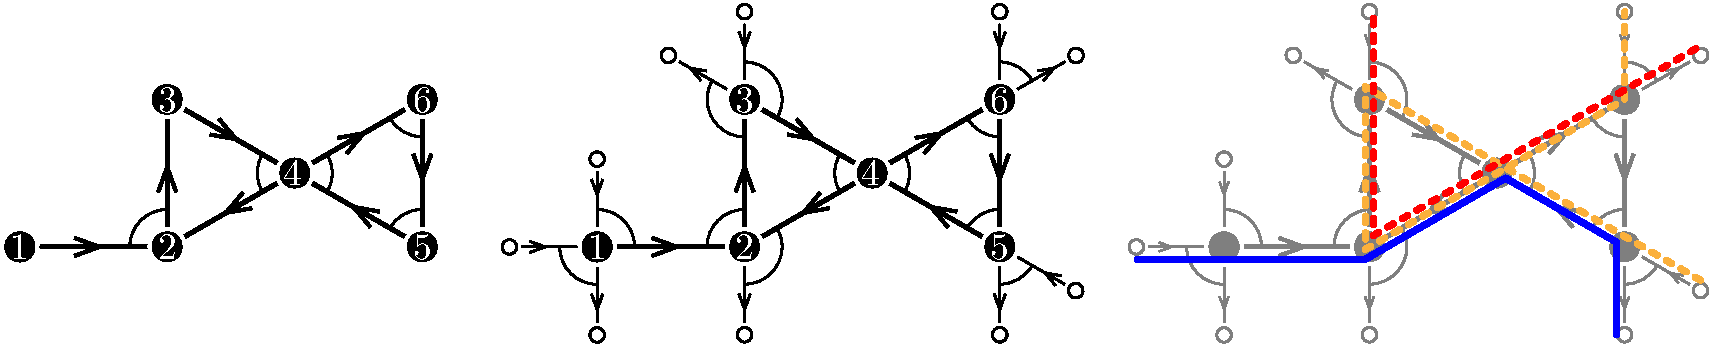
\includegraphics[scale=.6]{exmQuiver}}
	\caption{A gentle bound quiver~$\bar Q$ (left), its blossoming quiver~$\bar Q\blossom$ (middle), and some walks in~$\bar Q\blossom$ (right). The dotted red and orange walks are non-kissing, but both are kissing the plain blue walk. See Figure~\ref{fig:exmFlip} for examples of non-kissing facets.}
	\label{fig:exmQuiver}
\end{figure}

A \defn{walk} in~$\bar Q$ is a maximal string in~$\bar Q\blossom$, \ie connecting two vertices of~$Q_0\blossom \ssm Q_0$.
A walk~$\omega$ is \defn{bending} if it has two opposite arrows and \defn{straight} otherwise.
For~$v \in Q_0$, the \defn{peak walk}~$v_\peak$ (resp.~the \defn{deep walk}~$v_\deep$) is the walk with two outgoing (resp.~incoming) arrows at vertex~$v$ and one incoming and one outgoing arrow at all its other vertices.
A \defn{substring} of~$\omega = \omega_1^{\varepsilon_1} \dots \omega_\ell^{\varepsilon_\ell}$ is a factor~$\sigma = \omega_{m+1}^{\varepsilon_{m+1}} \dots \omega_{n-1}^{\varepsilon_{n-1}}$ with~$1 \le m < n \le \ell$.
We say that~$\sigma$ is a \defn{top} (resp.~\defn{bottom}) substring of~$\omega$ if~${\varepsilon_m = -1 = -\varepsilon_n}$ (resp.~${\varepsilon_m = 1 = -\varepsilon_n}$), meaning that~$\omega$ has two outgoing (resp.~incoming) arrows at the endpoints of~$\sigma$.
Let~$\Sigma_\bottom(\omega)$ and~$\Sigma_\top(\omega)$ be the sets of bottom and top substrings~of~$\omega$ respectively.

Consider two walks~$\omega,\omega'$ on~$\bar Q$.
We say that~$\omega$ \defn{kisses}~$\omega'$ if~$\Sigma_\top(\omega) \cap \Sigma_\bottom(\omega') \ne \varnothing$, \ie if there exists a common substring~$\sigma$ of~$\omega$ and~$\omega'$ such that~$\omega$ has two outgoing arrows incident to~$\sigma$ while~$\omega'$ has two incoming arrows incident to~$\sigma$.
See Figures~\ref{fig:exmQuiver}\,(right)~\&~\ref{fig:kissingFlip}\,(left).
We authorize the case where~$\sigma$ is reduced to a vertex~$v$, \ie~$v$ is a peak of~$\omega$ and a deep of~$\omega'$.
Note that~$\omega$ can kiss~$\omega'$ several times, that~$\omega$ and~$\omega'$ can mutually kiss, and that~$\omega$ can kiss itself.
The \defn{non-kissing complex} of~$\bar Q$ is the simplicial complex~$\NKC$ whose faces are the collections of walks which are not self-kissing and pairwise non-kissing.
Note that no straight walk can kiss another walk by definition, so that they appear in all facets of~$\NKC$.
We thus consider the \defn{reduced non-kissing complex}~$\RNKC$ to be the deletion of all straight walks from~$\NKC$.
See Figure~\ref{fig:exmNKC}\,(left).

Our definition of non-kissing complex is largely inspired from and specializes to simplicial complexes defined from subsets of the grid~\cite{PetersenPylyavskyySpeyer, SantosStumpWelker, McConville, GarverMcConville-grid} or from dissections of polygons~\cite{Baryshnikov, Chapoton-quadrangulations, GarverMcConville, MannevillePilaud-accordion}. 
To the best of our knowledge, we actually provide the first connection between these two families, besides the observation that associahedra are instances of both.
In fact, the example of Figure~\ref{fig:exmNKC} is also a special case of both families.

\begin{figure}[t]
	\centerline{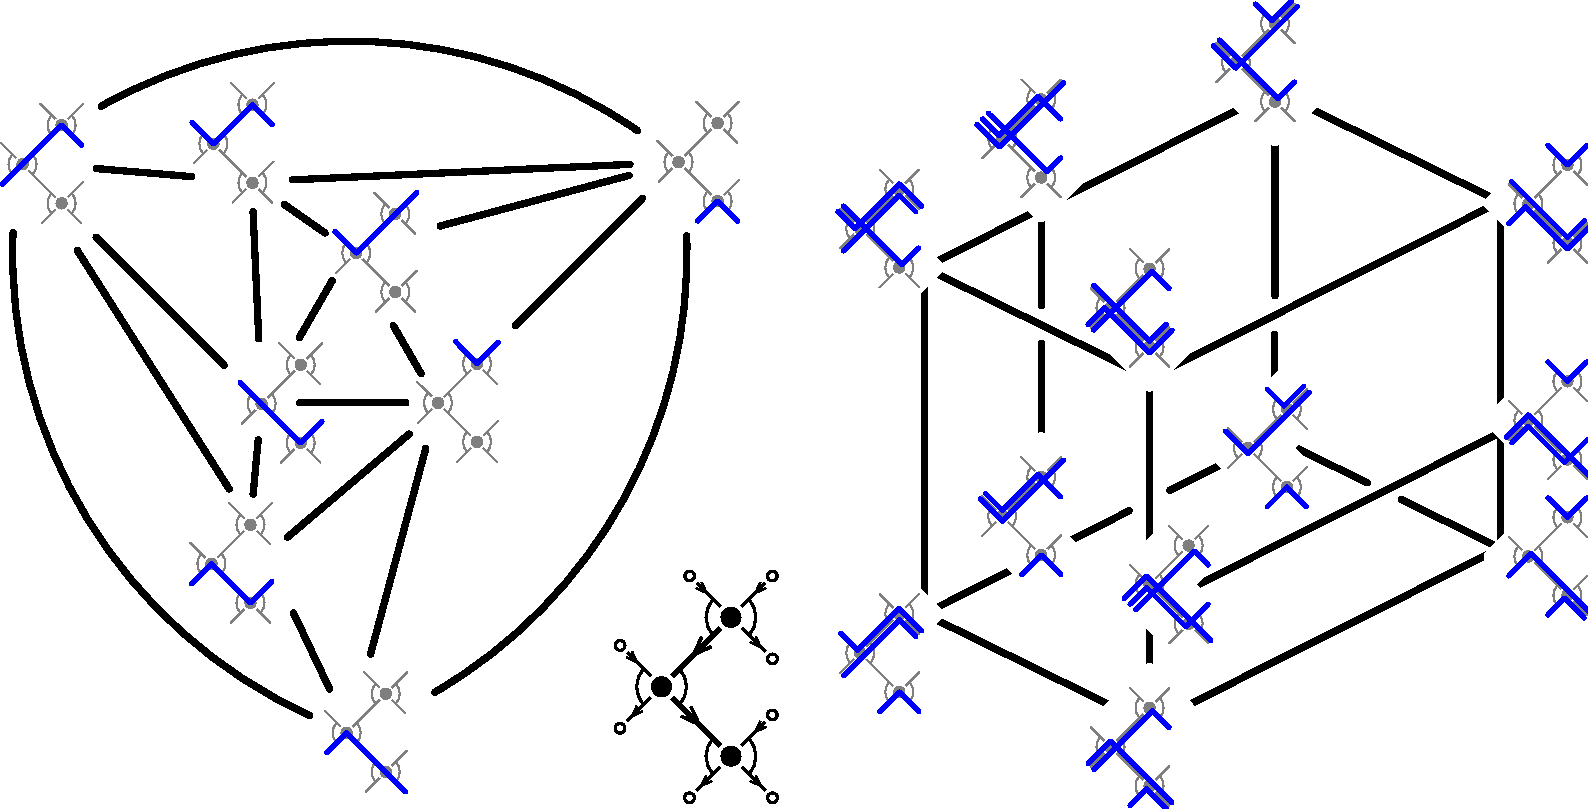
\includegraphics[scale=.59]{exmNKC}}
	\caption{A reduced non-kissing complex (left) and its flip graph~(right).}
	\label{fig:exmNKC}
\end{figure}

\begin{figure}[b]
	\centerline{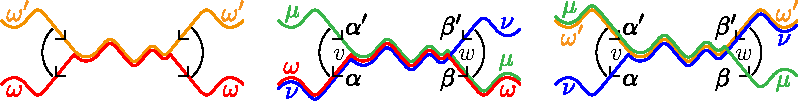
\includegraphics[scale=1.2]{kissingFlip}}
	\caption{Two kissing walks (left) and a flip~(right).}
	\label{fig:kissingFlip}
\end{figure}

\subsection{Distinguished arrows and flips}

We now show that the non-kissing complex~$\RNKC$ is a \defn{pseudomanifold}, \ie that it is \defn{pure} (all facets have the same dimension) and \defn{thin} (there is a well-defined notion~of~flips). 

A \defn{marked walk}~$\omega_\star$ is a walk~$\omega = \alpha_1^{\varepsilon_1} \cdots \alpha_\ell^{\varepsilon_\ell}$ with a marked arrow~$\alpha_i^{\varepsilon_i}$.
Consider two distinct non-kissing walks~$\mu_\star, \nu_\star$ marked at an arrow~$\alpha^\varepsilon \in Q\blossom_1$.
Let~$\sigma$ denote their maximal common substring containing that occurrence of~$\alpha$.
Since~$\mu_\star \ne \nu_\star$, their common substring~$\sigma$ is strict, so that~$\mu_\star$ and~$\nu_\star$ split at least at one endpoint of~$\sigma$.
We define the \defn{countercurrent order at~$\alpha$} by~$\mu_\star \prec_\alpha \nu_\star$ when~$\mu_\star$ enters and/or exits~$\sigma$ in the direction of~$\alpha$, while~$\nu_\star$ enters and/or exits~$\sigma$ in the opposite direction.
For a face~$F$ of~$\NKC$, we call \defn{distinguished walk} of~$F$ at an arrow~$\alpha$ the $\prec_\alpha$-maximal walk~$\distinguishedWalk{\alpha}{F}$, and we call \defn{distinguished arrows} of a walk~$\omega \in F$ the arrows~$\distinguishedArrows{\omega}{F} \eqdef \set{\alpha \in \omega}{\distinguishedWalk{\alpha}{F} = \omega}$.
The following statement is inspired from~\cite[Theorem~3.2]{McConville} and illustrated in Figure~\ref{fig:exmFlip}\,(left).

\begin{figure}[b]
	\centerline{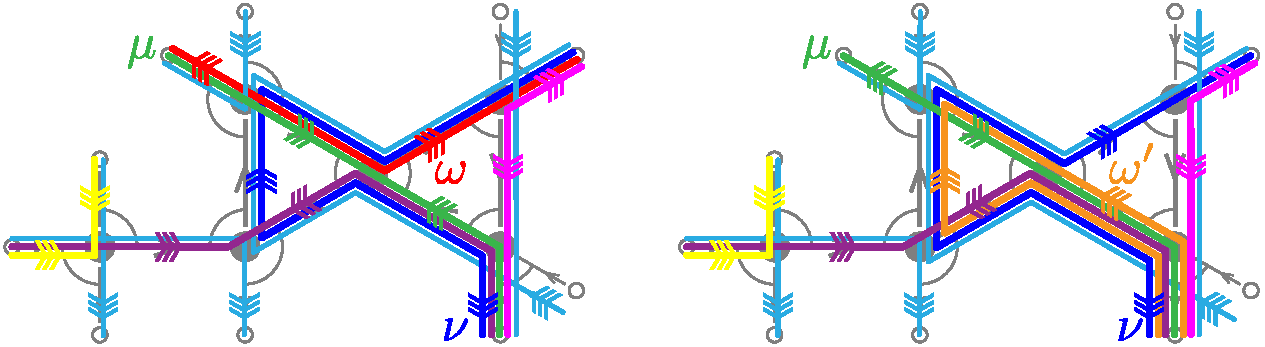
\includegraphics[scale=.68]{exmFlip}}
	\caption{Flipping the red walk~$\omega$ to the orange walk~$\omega'$. The walks~$\mu, \nu$ involved in the flip are the blue and green walks. Distinguished arrows are marked with triple~arrows.}
	\label{fig:exmFlip}
\end{figure}

\begin{proposition}
\label{prop:distinguishedArrows}
Each bending (resp.~straight) walk of a facet~$F \in \NKC$ contains precisely~$2$ (resp.~$1$) distinguished arrows pointing in opposite directions (resp.~in the direction~of~the~walk).
\end{proposition}

%The next statement follows by double counting (each arrow has a distinguished walk, while each bended/straight walk has two/one distinguished arrows).

\begin{corollary}
\label{coro:pure}
The reduced non-kissing complex~$\RNKC$ is pure of dimension~$|Q_0|$.
\end{corollary}

Define the \defn{distinguished string} of a bending walk~$\omega$ in a facet~$F \in \NKC$ as the substring~$\distinguishedString{\omega}{F}$ of~$\omega$ located between the two distinguished arrows of~$\omega$.

\begin{proposition}
\label{prop:flip}
Consider a facet~$F \in \NKC$ and a bending walk~$\omega \in F$.
Write~${\omega = \rho \sigma \tau}$ where~$\sigma \eqdef \distinguishedString{\omega}{F}$.
%The distinguished substring~$\sigma = \distinguishedString{\omega}{F}$ splits~$\omega$ into~${\omega = \rho \sigma \tau}$.
Let~$\{\alpha, \beta\} \eqdef \distinguishedArrows{\omega}{F}$, and~$\alpha'$ and~$\beta'$ be the other two arrows of~$Q_1\blossom$ incident to the endpoints of~$\sigma$ and such that~${\alpha'\alpha \in I}$ or~${\alpha\alpha' \in I}$, and ${\beta'\beta \in I}$ or~${\beta\beta' \in I}$.
Let~$\mu \eqdef \distinguishedWalk{\alpha'}{F \ssm \{\omega\}}$ and~$\nu \eqdef \distinguishedWalk{\beta'}{F \ssm \{\omega\}}$.
See Figures~\ref{fig:kissingFlip}\,(right) \&~\ref{fig:exmFlip}.~Then
\begin{compactenum}[(i)]
\item The string~$\sigma$ splits the walk~$\mu$ into~$\mu = \rho' \sigma \tau$ and the walk~$\nu$ into~$\nu = \rho \sigma \tau'$.
\item The walk~$\omega' \eqdef \rho' \sigma \tau'$ is kissing~$\omega$ but no other~walk~of~$F$. Moreover, $\omega'$ is the only other walk besides~$\omega$ which is not kissing any other walk of~$F \ssm \{\omega\}$.
\end{compactenum}
We say that~$F \symdif \{\omega, \omega'\}$ is obtained from~$F$ by \defn{flipping}~$\omega$, and that the flip is \defn{supported}~by~$\sigma$.
\end{proposition}

\begin{corollary}
The reduced non-kissing complex~$\RNKC$ is a pseudomanifold without boundary.
\end{corollary}

\newpage
\section{Non-kissing lattices}
\label{sec:nonkissinglattice}

The flip of Proposition~\ref{prop:flip} and Figures~\ref{fig:kissingFlip} \&~\ref{fig:exmFlip} exchanges two kissing walks~$\omega, \omega'$.
The~flip is \defn{increasing} when their common substring is on top of~$\omega$ and on the bottom of~$\omega'$.
This yields the \defn{increasing flip graph}, where vertices are non-kissing facets and arcs are increasing flips.
%The \defn{peak facet}~$\set{v_\peak}{v \in Q_0}$ is a source and the \defn{deep facet}~$\set{v_\deep}{v \in Q_0}$ is a sink.
See Figure~\ref{fig:exmNKC}\,(right).
The main result of this section is the following~statement.

\begin{theorem}
\label{thm:lattice}
If~$\RNKC$ is finite, the increasing flip graph is the Hasse diagram of a congruence-uniform lattice, that we call \defn{non-kissing lattice} and denote by~$\NKL$.
\end{theorem}

Congruence-uniform lattices will be properly defined in Section~\ref{subsec:joinRepresentations}.
To achieve Theorem~\ref{thm:lattice}, we use a technique developed by T.~McConville for grid quivers~\cite{McConville}: we identify the non-kissing lattice with a quotient of a lattice of biclosed sets of strings.

\subsection{Biclosed sets of strings}
\label{subsec:biclosedSets}

A \defn{closure operator} on a finite set~$\cS$ is a map~$S \mapsto \closure{S}$ on subsets of~$\cS$ such that~$\closure{\varnothing} = \varnothing$, $S \subseteq \closure{S}$, $\closure{(\closure{S})} = \closure{S}$ and~$S \subseteq T \Longrightarrow \closure{S} \subseteq \closure{T}$ for any~$S,T \subseteq \cS$.
A subset~${S \subseteq \cS}$ is \defn{closed} if~$\closure{S} = S$, \defn{coclosed} if~$\cS \ssm S$ is closed, and \defn{biclosed} if it is both closed and coclosed.
Let~$\Bicl{\cS}$ be the inclusion poset of biclosed subsets of~$\cS$.
In~\cite[Theorem~5.5]{McConville}, T.~McConville gave simple sufficient conditions for~$\Bicl{\cS}$ to be a congruence uniform lattice.
In~\cite[Theorem~3.21]{PaluPilaudPlamondon}, we extended this criterion in the situation when the singletons of~$\cS$ are not biclosed so that we can apply it in our context of non-kissing complexes.

In a gentle bound quiver~$\bar Q$, we define the \defn{closure}~$\closure{S}$ of a set~$S$ of strings of~$\bar Q$ as the set of all strings of the form~$\sigma_1 \alpha_1^{\varepsilon_1} \sigma_2 \alpha_2^{\varepsilon_2} \dots \alpha_{\ell-1}^{\varepsilon_{\ell-1}} \sigma_\ell$ where~$\sigma_i \in S, \alpha_i \in Q_1$ and~${\varepsilon_i \in \{-1,1\}}$.
Let~$\Bicl{\bar Q}$ be the inclusion poset on biclosed sets of strings of~$\bar Q$.
For example, when~$\bar Q$ is a path on $n$ vertices with no relation, the strings are in bijection with pairs~${(i,j) \in \binom{n+1}{2}}$, the closure on strings translates to the concatenation~${(i,j) \circ (k,\ell) = \delta_{j = k} (i, \ell)}$, biclosed sets of strings are in bijection with inversion sets of permutations of~$[n+1]$, so that~$\Bicl{\bar Q}$ is isomorphic to the weak order on~$\fS_{n+1}$.
Figure~\ref{fig:exmLatticeQuotient}\,(left) illustrates the poset~$\Bicl{\bar Q}$ for another gentle bound quiver, with the empty set in the bottom and the set of all strings of~$\bar Q$ on top. The criterion of~\cite[Theorem~3.21]{PaluPilaudPlamondon} yields the following~result.

\begin{theorem}
When~$\bar Q$ has finitely many strings, the inclusion poset of biclosed sets~$\Bicl{\bar Q}$ is a congruence-uniform lattice.

\begin{figure}[t]
	\centerline{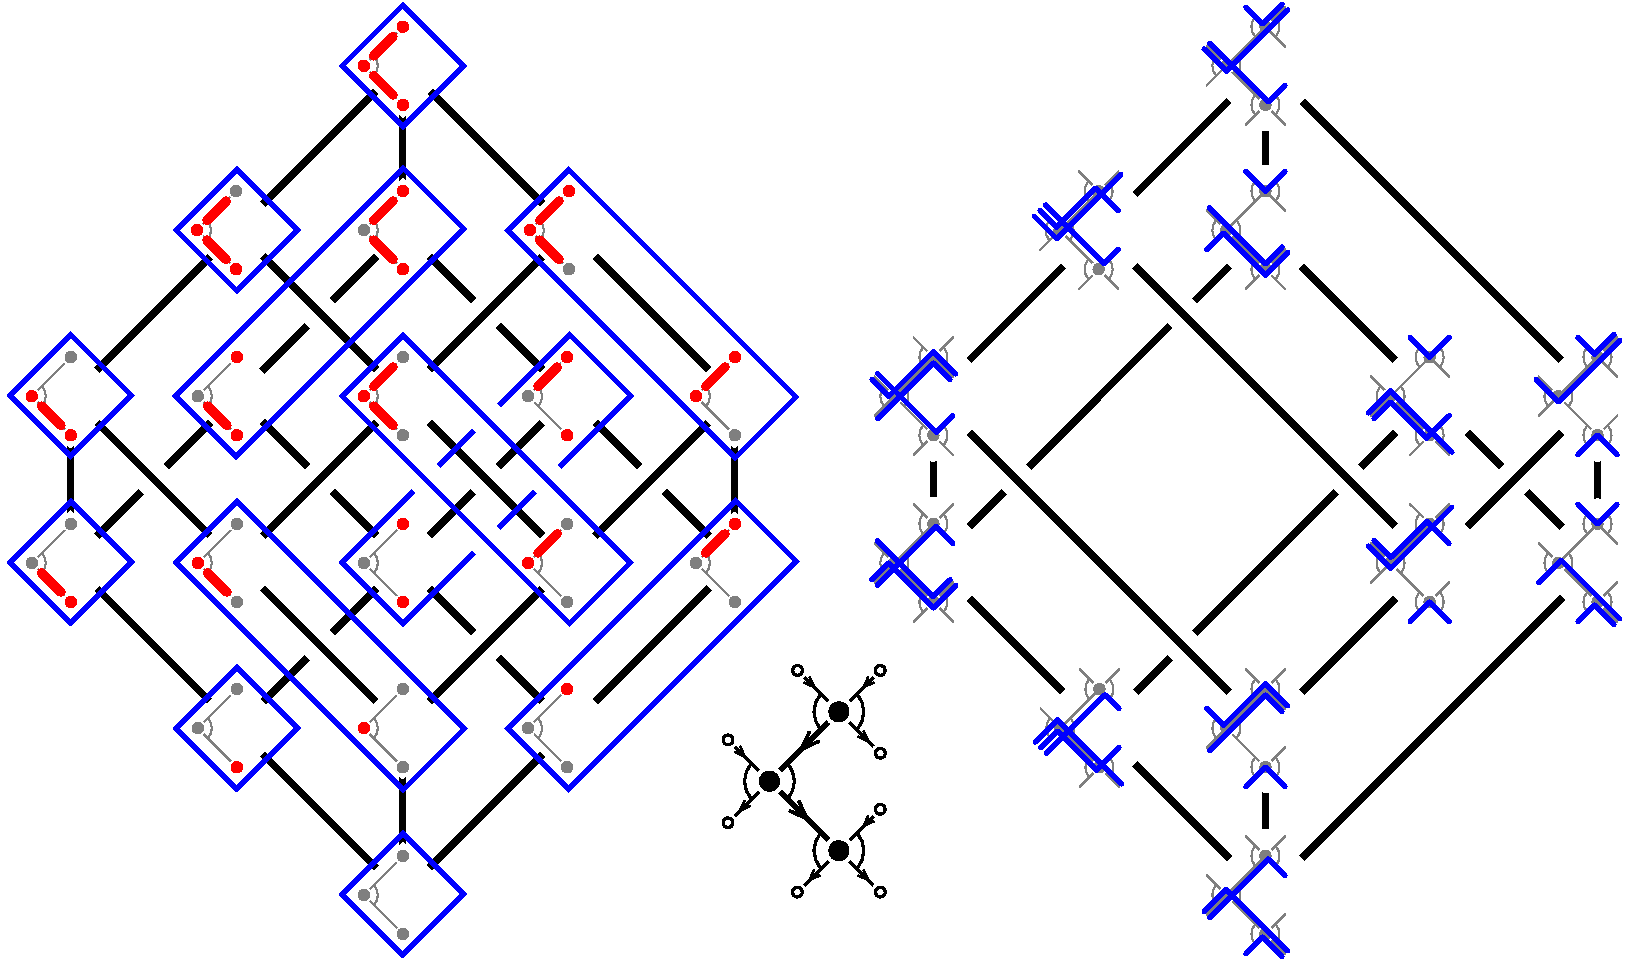
\includegraphics[scale=.59]{exmLatticeQuotient}}
	\caption{The inclusion lattice of biclosed sets~$\Bicl{\bar Q}$ with congruence classes of~$\equiv$ in blue (left), and the corresponding lattice of increasing flips on facets of~$\NKC$ (right).}
	\label{fig:exmLatticeQuotient}
\end{figure}
\end{theorem}

\subsection{Lattice congruence}
\label{subsec:congruence}

A \defn{lattice congruence} of a lattice~$(L, \le, \meet, \join)$ is an equivalence relation~$\equiv$ on~$L$ compatible with meets and joins: $x \equiv x'$ and~$y \equiv y'$ implies~$x \meet y \equiv x' \meet y'$ and~$x \join y \equiv x' \join y'$. 
It defines a \defn{lattice quotient}~$L/{\equiv}$ on the congruence classes of~$\equiv$ where the order relation is given by~$X \le Y$ iff there exists~$x \in X$ and~$y \in Y$ such that~$x \le y$ and the meet~$X \meet Y$ (resp.~the join~$X \join Y$) of two congruence classes~$X$ and~$Y$ is the congruence class of~$x \meet y$ (resp.~of~$x \join y$) for arbitrary representatives~$x \in X$~and~$y \in Y$.
For a finite lattice~$L$, an equivalence relation~$\equiv$ on~$L$ is a lattice congruence if and only if its congruence classes are intervals and the maps~$\projDown$ and~$\projUp$, sending an element~$x \in L$ to the minimum and maximum of its congruence class respectively, are order preserving.
%In fact, one can also define a lattice congruence directly by its up and down maps~$\projUp$~and~$\projDown$.

Following~\cite[Section~7]{McConville}, we associate to a biclosed set~$S \in \Bicl{\bar Q}$ the sets \\[.1cm]
\centerline{$
\projDown(S) \eqdef \set{\sigma \in \strings(\bar Q)}{\Sigma_\bottom(\sigma) \subseteq S}
\quad\text{and}\quad
\projUp(S) \eqdef \set{\sigma \in \strings(\bar Q)}{\Sigma_\top(\sigma) \cap S \ne \varnothing}.
$} \\[.1cm]
Here and throughout the paper, we denote by~$\Sigma_\bottom(\sigma)$ the set of bottom substrings for a string ${\sigma = \alpha_1^{\varepsilon_1} \dots \alpha_\ell^{\varepsilon_\ell}}$, \ie the substrings~$\alpha_m^{\varepsilon_m} \dots \alpha_n^{\varepsilon_n}$ for $1 \le m \le n \le \ell$ such that~$m = 1$ or~$\varepsilon_{m-1} = -1$, and $n = \ell$ or $\varepsilon_{n+1} = 1$ (and similarly for the set of top substrings~$\Sigma_\top(\sigma)$).

\begin{proposition}
\label{prop:latticeCongruence}
For any~$S \in \Bicl{\bar Q}$, the sets~$\projDown(S)$ and~$\projUp(S)$ are biclosed.
Moreover,
\begin{compactenum}[(i)]
\item
$\projDown(S) \subseteq S \subseteq \projUp(S)$ for any element~$S \in \Bicl{\bar Q}$,

\item
$\projDown \circ \projDown = \projDown \circ \projUp = \projDown$ and $\projUp \circ \projUp = \projUp \circ \projDown = \projUp$,

\item
$\projDown$ and~$\projUp$ are order preserving.
\end{compactenum}
Therefore, the fibers of~$\projUp$ and~$\projDown$ coincide and are the classes of a lattice congruence~$\equiv$ on~$\Bicl{\bar Q}$.
\end{proposition}

For example, if~$\bar Q$ is an oriented path with no relation, $\equiv$ is a Cambrian congruence of the weak~order~\cite{Reading-CambrianLattices}.
The congruence classes of~$\equiv$ appear as blue rectangles~in~Figure~\ref{fig:exmLatticeQuotient}.

\subsection{Non-kissing lattice}

Coming back to our original problem, we now aim to show that the increasing flip graph on non-kissing facets is isomorphic to the Hasse diagram of the quotient of the lattice of biclosed set~$\Bicl{\bar Q}$ of Section~\ref{subsec:biclosedSets} by the lattice congruence of Section~\ref{subsec:congruence}.
The next two propositions provide explicit maps between biclosed sets of strings and non-kissing facets illustrated in Figure~\ref{fig:exmSurjection}. It extends previous definitions of~\cite{McConville} for grid quivers.

\begin{proposition}
For~$S \in \Bicl{\bar Q}$ and~$\alpha \in Q_1\blossom$, let
\(
{\omega(\alpha,S) \eqdef \alpha_{-\ell}^{\varepsilon_{-\ell}} \cdots \alpha_{-1}^{\varepsilon_{-1}} \cdot \alpha \cdot \alpha_1^{\varepsilon_1} \cdots \alpha_r^{\varepsilon_r}}
\)
be the directed walk containing~$\alpha$ defined by
\begin{compactitem}
\item $\varepsilon_i = -1$ if the string~$\alpha_1^{\varepsilon_1} \cdots \alpha_{i-1}^{\varepsilon_{i-1}}$ belongs to~$S$, and~$\varepsilon_i = 1$ otherwise, for all~$i \in [r]$,
\item $\varepsilon_{-i} = 1$ if the string~$\alpha_{-i+1}^{\varepsilon_{-i+1}} \cdots \alpha_{-1}^{\varepsilon_{-1}}$ belongs to~$S$, and~$\varepsilon_i = -1$ otherwise, for all~$i \in [\ell]$.
\end{compactitem}
Then the set~$\set{\omega(\alpha,S)}{\alpha \in Q_1\blossom}$ contains~$2|Q_0| - |Q_1|$ straight walks and~$|Q_0|$~pairs of inverse directed bending walks, which are all pairwise non-kissing.
We thus obtain a facet~$\eta(S)$ of~$\NKC$ by identifying these pairs of inverse directed bending walks.
\end{proposition}

\begin{proposition}
For any facet~$F \in \NKC$, the set~$\zeta(F) \eqdef \displaystyle\closure{\Big( \bigcup\limits_{\omega \in F} \Sigma_\bottom(\omega) \Big)}
$~is~biclosed.
\end{proposition}

When the quiver is an oriented path with no relation, the map~$\eta$ should be thought of as the map from permutations to triangulations defined in~\cite{Reading-CambrianLattices}.
Conversely, $\zeta$ maps a triangulation to the minimal permutation in its fiber under~$\eta$.
For the straight quiver, $\eta$ plays the role of the binary search tree insertion while~$\zeta$ selects the minimal linear extension of a binary tree.
%
Using these maps, we show that the increasing flip graph on non-kissing facets is isomorphic to the Hasse diagram of the lattice quotient~$\Bicl{\bar Q}/{\equiv}$.

\begin{theorem}
The maps~$\eta: \Bicl{\bar Q} \to \NKC$ and~$\zeta: \NKC \to \Bicl{\bar Q}$ satisfy:
\begin{compactitem}
\item $\eta \big( \zeta(F) \big) = F$ for any facet~$F \in \NKC$,
\item $\zeta \big( \eta(S) \big) = \projDown(S)$ for any biclosed set~$S \in \Bicl{\bar Q}$,
\item for any facet~$F' \in \RNKC$ and~$\sigma \in \zeta(F')$, there exists an increasing flip~$F \to F'$ supported by~$\sigma$ if and only if~$\zeta(F') \ssm \{\sigma\}$ is biclosed.
\end{compactitem}
Therefore, the facets of~$\NKC$ are in bijection with the congruence classes of~$\equiv$ and the increasing flip graph is the Hasse diagram of the lattice quotient~$\Bicl{\bar Q}/{\equiv}$.

\begin{figure}[b]
	\vspace{-.3cm}
	\centerline{
	\begin{overpic}[scale=.5]{exmSurjection}
			\put(28,8){$\longrightarrow$}
			\put(29,10){$\eta$}
			\put(69,8){$\longrightarrow$}
			\put(70,10){$\zeta$}
			\put(13,-3){$S$}
			\put(46,-3){$\eta(S)$}
			\put(77,-3){$\zeta(\eta(S)) = \projDown(S)$}
	\end{overpic}
	}
	\vspace{.4cm}
	\caption{The maps~$\eta$ (left) and $\zeta$ (right) between non-kissing facets and biclosed sets.}
	\label{fig:exmSurjection}
\end{figure}
\end{theorem}

\newpage
\subsection{Canonical join complex}
\label{subsec:joinRepresentations}

In a lattice~$(L,\le,\meet,\join)$, a \defn{join representation} of~$x \in L$ is a subset~$J \subseteq L$ such that~${x = \bigJoin J}$.
This representation is \defn{irredundant} if~$x \ne \bigJoin J'$ for a strict subset~$J' \subsetneq J$.
The irredundant join representations of~$x \in L$ are ordered by containement of the lower ideals of their elements, \ie~$J \le J'$ if and only if for any~$y \in J$ there exists~$y' \in J'$ such that~$y \le y'$.
When this order has a minimal element, it is called the \defn{canonical join representation} of~$x$.
All elements of the canonical join representation~$x = \bigJoin J$ are then \defn{join-irreducible}, \ie cover a single element. Canonical meet representations and meet-irreducibles are defined dually.

A lattice~$L$ is \defn{congruence-uniform} if its join-irreducible elements are in bijection with the join-irreducibles of its lattice of congruences, and similarly for meet-irreducibles.
Congruence-uniform lattices behave nicely with join representations and congruence lattices.
In particular, congruence-uniform lattices are semi-distributive, so that any element admits a canonical join representation.
The collection of sets~$J$ which define canonical join representations in~$L$ is the \defn{canonical join complex} of~$L$.

To conclude our study of the non-kissing lattice~$\NKL$, we describe its canonical join complex.
We say that a string~$\sigma \in \strings(\bar Q)$ is \defn{distinguishable} if there is a facet~${F \in \NKC}$ and a walk~$\omega \in F$ such that~$\sigma = \distinguishedString{\omega}{F}$.
These strings are characterized as follows.

\begin{proposition}
\label{prop:characterizationDistinguishableStrings}
A string~$\sigma \in \strings(\bar Q)$ is distinguishable if and only if ${\Sigma_\bottom(\sigma) \cap \Sigma_\top(\sigma) = \{\sigma\}}$.
\end{proposition}

One checks that~$\closure{\Sigma_\bottom(\sigma)}$ is biclosed so that we can define~$\ji(\sigma) \eqdef \eta \big( \closure{\Sigma_\bottom(\sigma)} \big)$.

\begin{proposition}
The map~$\ji : \sigma \mapsto \ji(\sigma)$ defines a bijection between the distinguishable strings of~$\bar Q$ and the join-irreducible elements of the non-kissing lattice~$\NKL$.
\end{proposition}

Therefore, distinguishable strings are building blocks for canonical join representations in~$\NKL$.
A \defn{descent} of a facet~$F \in \NKC$ is a string~$\sigma$ which is the distinguished string of a walk~$\omega$ of~$F$ and is a bottom substring of~$\omega$ (so that the flip of~$\omega$ in~$F$ is a descent in the non-kissing lattice).
We denote by~$\descents(F)$ the set of descents of~$F$.

\begin{proposition}
The canonical join representation of~$F \in \NKL$ is given by ${F = \!\!\! \bigJoin\limits_{\sigma \in \descents(F)} \!\!\! \ji(\sigma)}$.
\end{proposition}

To conclude, we characterize which subsets of strings correspond to canonical join representations in the non-kissing lattice~$\NKL$.
Following~\cite{GarverMcConville-grid}, we say that two strings are \defn{non-friendly} if $\Sigma_\top(\sigma) \cap \Sigma_\bottom(\tau) = \varnothing = \Sigma_\bottom(\sigma) \cap \Sigma_\top(\tau)$.
We call \defn{non-friendly complex} the simplicial complex of sets of pairwise non-friendly distinguishable strings.

\begin{theorem}
The following assertions are equivalent for a set~$\Sigma$ of distinguishable strings~of~$\bar Q$:
\begin{compactitem}
\item Any two strings of~$\Sigma$ are non-friendly.
\item $\set{\ji(\sigma)}{\sigma \in \Sigma}$ is the canonical join-representation of a facet of~$\NKC$.
\item $\Sigma$ is the descent set of a non-kissing facet~$F \in \NKC$.
\end{compactitem}
In other words, the canonical join complex of~$\NKL$ is isomorphic to the non-friendly complex.
\end{theorem}

For example, when the quiver is a straight path with no relation, the non-friendly complex is isomorphic to the non-crossing partition complex.

\newpage
\section{Gentle associahedra}
\label{sec:gentleAssociahedra}

In this section, we provide polyhedral realizations for finite non-kissing complexes, using tools inspired from the finite type cluster algebras of S.~Fomin and A.~Zelevinsky~\cite{FominZelevinsky-ClusterAlgebrasII}.

\subsection{$\b{g}$-vectors and $\b{c}$-vectors}

Let~${\multiplicityVector_V \eqdef \sum_{i \in [m]} \b{e}_{v_i} \in \R^{Q_0}}$ be the \defn{multiplicity vector} of a multiset~$V = \{v_1, \dots, v_m\}$ of~$Q_0$.
For a string~$\sigma \in \strings(\bar Q)$, let~$\multiplicityVector_\sigma \eqdef \multiplicityVector_{V(\sigma)}$ where~$V(\sigma)$ is the multiset of vertices~of~$\sigma$. 

For a walk~$\omega$ on~$\bar Q$, we denote by~$\peaks{\omega}$ (resp.~by~$\deeps{\omega}$) the (multi)set of peaks (resp.~deeps) of~$\omega$.
The \defn{$\b{g}$-vector} of~$\omega$ is the vector~${\gvector{\omega} \eqdef \multiplicityVector_{\peaks{\omega}} - \multiplicityVector_{\deeps{\omega}} \in \R^{Q_0}}$.
For a set~$\Omega$ of walks, $\gvectors{\Omega} \eqdef \! \set{\gvector{\omega}\!}{\!\omega \in \Omega}$.
Note that~$\gvector{\omega} = 0$ for a straight~walk~$\omega$.

Consider a bending walk~$\omega$ in a facet~$F \in \RNKC$.
By Proposition~\ref{prop:distinguishedArrows}, $\omega$ has two~distinguished arrows~$\distinguishedArrows{\omega}{F}$ around its distinguished string~$\distinguishedString{\omega}{F}$.
\mbox{The \defn{$\b{c}$-vector} of~$\omega \in F$} is the vector~${\cvector{\omega}{F} \eqdef \distinguishedSign{\omega}{F} \, \multiplicityVector_{\distinguishedString{\omega}{F}} \in \R^{Q_0}}$, where~$\distinguishedSign{\omega}{F} \eqdef 1$ if~${\distinguishedString{\omega}{F} \in \Sigma_\top(\omega)}$ and $\distinguishedSign{\omega}{F} \eqdef -1$ if~${\distinguishedString{\omega}{F} \in \Sigma_\bottom(\omega)}$.
Denote by~$\cvectors{F} \eqdef \set{\cvector{\omega}{F}}{\omega \in F}$.

\begin{proposition}
\label{prop:gvectorscvectorsDualBases}
For any non-kissing facet~$F \in \RNKC$, the set of $\b{g}$-vectors~$\gvectors{F}$ and the set of $\b{c}$-vectors~$\cvectors{F}$ form dual bases.
%
\begin{figure}[h]
	\centerline{$\raisebox{-1.5cm}{\begin{overpic}[scale=.65]{exmVectors}\put(60,-4){$F$}\end{overpic}}$ \quad \(
\begin{blockarray}{ccccccc}
	& {\color{red} \bullet} & {\color{orange} \bullet} & {\color{yellow} \bullet} & {\color{green} \bullet} & {\color{blue} \bullet} & {\color{violet} \bullet} \\
	\begin{block}{c(cccccc)}
	1 & 0 & 0 & 0 & 0 & 0 & \!\!-1\\
	2 & 0 & 0 & 0 & 0 & \!\!-1\!\! & 0 \\
	3 & 0 & 1 & 0 & 1 & 0 & 0 \\
	4 & 0 & 0 & 0 & \!\!-1\!\! & 0 & 0 \\
	5 & 0 & 0 & 1 & 1 & 1 & 0 \\
	6 & 1 & 0 & 0 & 0 & 0 & 0 \\
	\end{block}
	& & & \multicolumn{2}{c}{$\gvectors{F}$} & &
\end{blockarray}
%
\qquad
%
\begin{blockarray}{ccccccc}
	& {\color{red} \bullet} & {\color{orange} \bullet} & {\color{yellow} \bullet} & {\color{green} \bullet} & {\color{blue} \bullet} & {\color{violet} \bullet} \\
	\begin{block}{c(cccccc)}
	1 & 0 & 0 & 0 & 0 & 0 & \!\!-1 \\
	2 & 0 & 0 & 1 & 0 & \!\!-1\!\! & 0 \\
	3 & 0 & 1 & 0 & 0 & 0 & 0 \\
	4 & 0 & 1 & 1 & \!\!-1\!\! & 0 & 0 \\
	5 & 0 & 0 & 1 & 0 & 0 & 0 \\
	6 & 1 & 0 & 0 & 0 & 0 & 0 \\
	\end{block}
	& & & \multicolumn{2}{c}{$\cvectors{F}$} & &
\end{blockarray}
\)}
	\vspace{-.3cm}
	\caption{The $\b{g}$- and $\b{c}$-matrices of a facet~$F$ form dual bases.}
	\vspace{-.7cm}
	\label{fig:gcvectors}
\end{figure}
\end{proposition}

\subsection{$\b{g}$-vector fans and gentle associahedra}

We now use $\b{g}$- and~$\b{c}$-vectors to construct polyhedral realizations of finite non-kissing complexes.
Since the $\b{g}$-vectors of the walks~$\omega, \omega', \mu, \nu$ involved in the flip of Figure~\ref{fig:kissingFlip} satisfy the linear dependence $\gvector{\omega} + \gvector{\omega'} = \gvector{\mu} + \gvector{\nu}$, we get the following~statement.

\begin{theorem}
\label{thm:gvectorFan}
For a gentle bound quiver~$\bar Q$ with finite non-kissing complex~$\RNKC$, the collection of cones
\(
\gvectorFan \eqdef \set{\R_{\ge0} \gvectors{F}}{F \text{ non-kissing face of } \RNKC}
\)
forms a complete simplicial fan, that we call the \defn{$\b{g}$-vector fan} of~$\bar Q$.
\end{theorem}

\begin{figure}[h]
	\centerline{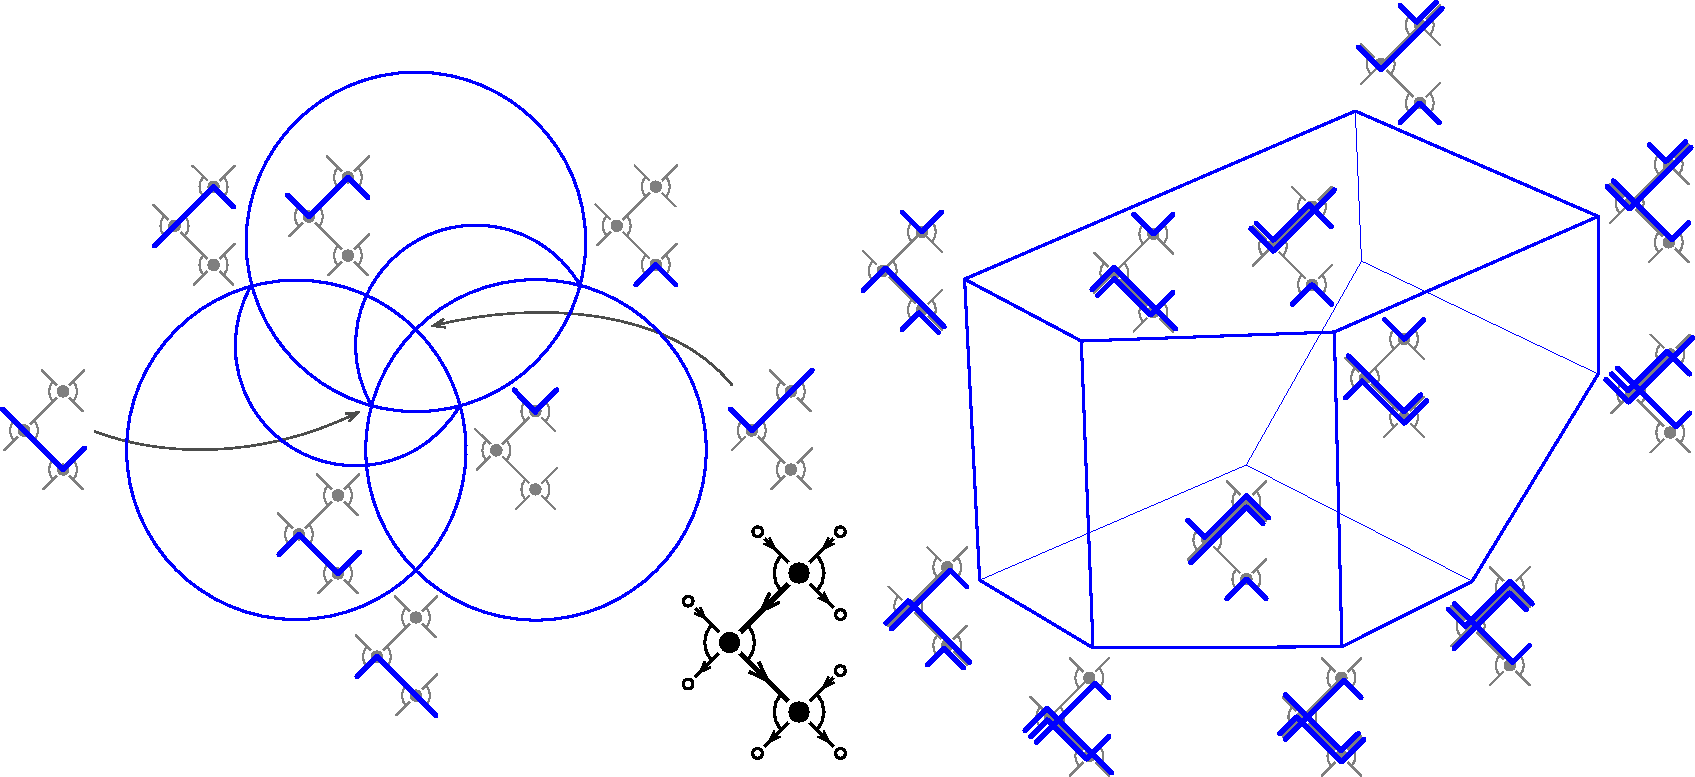
\includegraphics[scale=.59]{exmFanAsso}}
	\caption{The $\b{g}$-vector fan~$\gvectorFan$ (left) and the gentle associahedra (right).}
	\label{fig:exmFans}
\end{figure}

This fan is illustrated in Figure~\ref{fig:exmFans}\,(left).
Note that it was constructed in~\cite{MannevillePilaud-accordion} for dissection quivers and in~\cite{GarverMcConville-grid} for grid quivers. Both constructions extend the type~$A$ Cambrian fans of N.~Reading and D.~Speyer~\cite{ReadingSpeyer} obtained for path~quivers with no relations.

\newpage
We now aim at constructing a polytope whose normal fan is the $\b{g}$-vector fan of~$\bar Q$.
For two walks~$\omega, \omega'$ on~$\bar Q$, denote by~$\kn(\omega,\omega')$ the number of distinct kisses of~$\omega$ to~$\omega'$.
%Note that kisses are counted with multiplicities if~$\omega$ or~$\omega'$ pass twice through the same substring.
The \defn{kissing number} of~$\omega$ and~$\omega'$ is~$\KN(\omega,\omega') \eqdef \kn(\omega,\omega') + \kn(\omega',\omega)$.
When~$\RNKC$ is finite, we can define the \defn{kissing number} of a walk~$\omega$ on~$\bar Q$ as
\(
\KN(\omega) \eqdef \sum_{\omega'} \KN(\omega,\omega').
\)
%where the sum runs over all walks~$\omega'$ on~$\bar Q$.
%We obtain the following statement.

%\begin{theorem}
%\label{thm:associahedron}
%Let~$\bar Q$ be a gentle bound quiver with finite non-kissing complex~$\RNKC$.
%Define
%\begin{compactenum}[(i)]
%\item a point
%\(
%\point{F} \eqdef \sum_{\omega \in F} \KN(\omega) \, \cvector{\omega}{F}
%\)
%for each non-kissing facet~${F \in \RNKC}$,
%\item a halfspace
%\(
%\HS{\omega} \eqdef \bigset{\b{x} \in \R^{Q_0}}{\dotprod{\gvector{\omega}}{\b{x}} \le \KN(\omega)}
%\)
%for each walk~$\omega$ on~$\bar Q$.
%\end{compactenum}
%Then the two sets of~$\R^{Q_0}$ given by
%\begin{compactenum}[(i)]
%\item the convex hull of the points~$\point{F}$ for all non-kissing facets~${F \in \RNKC}$,
%\item the intersection of the halfspaces~$\HS{\omega}$ for all walks~$\omega$ on~$\bar Q$,
%\end{compactenum}
%define the same polytope whose normal fan is the $\b{g}$-vector fan~$\gvectorFan$.
%We call this polytope the \defn{$\bar Q$-associahedron} and denote it by~$\Asso$.
%\end{theorem}

\begin{theorem}
\label{thm:associahedron}
For a gentle bound quiver~$\bar Q$ with finite non-kissing complex~$\RNKC$, the $\b{g}$-vector fan~$\gvectorFan$ is the normal fan of the \defn{$\bar Q$-associahedron}~$\Asso$ defined equivalently as:
\begin{compactenum}[(i)]
\item the convex hull of the points~$\point{F} \eqdef \sum_{\omega \in F} \KN(\omega) \, \cvector{\omega}{F}$ for all facets~${F \in \RNKC}$,~or
\item the intersection of the halfspaces~$\HS{\omega} \eqdef \bigset{\b{x} \in \R^{Q_0}}{\dotprod{\gvector{\omega}}{\b{x}} \le \KN(\omega)}$ for all walks~$\omega$ on~$\bar Q$.
\end{compactenum}
\end{theorem}

For path quivers with no relation, we recover the associahedra of C.~Hohlweg and C.~Lange~\cite{HohlwegLange}.
The latter are obtained by deleting inequalities in the facet description of the classical permutahedron.
This property is lost for arbitrary gentle quivers: on the one hand, the Coxeter arrangement supporting the $\b{g}$-vector fan~$\gvectorFan$ is not necessarily of finite type; on the other hand, the $\bar Q$-associahedron is not always obtained by deleting inequalities in the facet description of the Minkowski sum of all $\b{c}$-vectors. See~\cite{PaluPilaudPlamondon} for a detailed discussion.
The $\bar Q$-associahedron was constructed in~\cite{MannevillePilaud-accordion} in the special case of dissection quivers.
An example of~$\Asso$ is shown in Figure~\ref{fig:exmFans}.
%The $\bar Q$-associahedron was constructed in~\cite{MannevillePilaud-accordion} in the special case of dissection quivers, generalizing the associahedra of C.~Hohlweg and C.~Lange~\cite{HohlwegLange} for path quivers with no relations.
%An example of~$\Asso$ is illustrated in Figure~\ref{fig:exmFans}. 
For grid quivers, our construction proves the polytopality conjecture for the $\b{g}$-vector fan stated~in~\cite{GarverMcConville-grid}.

This realization of the non-kissing complex has the following relevant property regarding the non-kissing lattice studied in Section~\ref{sec:nonkissinglattice}.

\begin{proposition}
When oriented in the linear direction~$(-1, \dots, -1) \in \R^{Q_0}$, the graph of the $\bar Q$-associahedron is (isomorphic to) the increasing flip graph.
\end{proposition}

%% if you use biblatex then this generates the bibliography
%% if you use some other method then remove this and do it your own way
\printbibliography

\end{document}
